\documentclass{article}
\usepackage{preamble}

\DeclareCaptionType{equ}[][]
\captionsetup{width=\linewidth}

\title{Eclectronics Mini-Project 1 Analysis and Design Choices}
\author{Jacob Smilg}
\date{September 15 2022}

\begin{document}

\maketitle

\section{Circuit Design Choices}

\begin{figure}[!ht]
    \centering
    \includesvg[width=.9\columnwidth]{images/kicad_schem.svg}
    \caption{The schematic of my circuit in KiCad.}
    \label{fig:kicad_schem}
\end{figure}

When designing my circuit for this mini-project, I began with a hysteretic oscillator since it's simple and uses a minimal number of components. This required me to generate a separate voltage \(V_{ref}\) in addition to the \qty{3.3}{\volt} regulator output. This is formed by sending the output of a voltage divider created by R1 and R2 through a unity-gain buffer. This buffer prevents \(V_{ref}\) from fluctuating with \(V_{out}\). The output of the oscillator is connected to the current-limiting resistor R6, which is connected to a red LED. I also placed bypass capacitors on the power pins of the op-amp and voltage regulator according to their datasheets.

With the essential structure out of the way, I began selecting component values that would keep the period of oscillation \(T\) within \(\pm10\%\) of 1 second. I did this based on equation 4.16 from the provided draft copy of \textit{Another Book on Circuits}:

\begin{equation}
    T=\tau\log\frac{V_{dd}-\alpha\left(V_{dd}-V_{ref}\right)}{\alpha\left(V_{dd}-V_{ref}\right)}\frac{V_{dd}-\alpha V_{ref}}{\alpha V_{ref}}
    \label{eq:period}
\end{equation}

In this case, \(\alpha=R_4/\left(R_4+R_5\right)\), \(V_{dd}=\qty{3.3}{\volt}\), \(V_{ref}=V_{dd}*R_2/\left(R_1+R_2\right)\), and \(\tau=R_3*C_1\). To start, I figured that \(\tau\) would have the largest effect on \(T\), followed by \(\alpha\) with a smaller effect, and \(V_{ref}\) having a relatively minor effect. Thus, my approach would be finding values for R3 and C1 that result in a nominal period close to 1 second using voltage divider ratios of 0.5 for \(\alpha\) and \(V_{ref}\) (resulting in \(V_{ref}=\qty{1.65}{\volt}\)). To do this, I created a spreadsheet with a matrix of all of the allowed component values to calculate the period for all combinations of a single resistor and capacitor (Figure~\ref{fig:spreadsheet}). 

\begin{figure}[!ht]
    \centering
    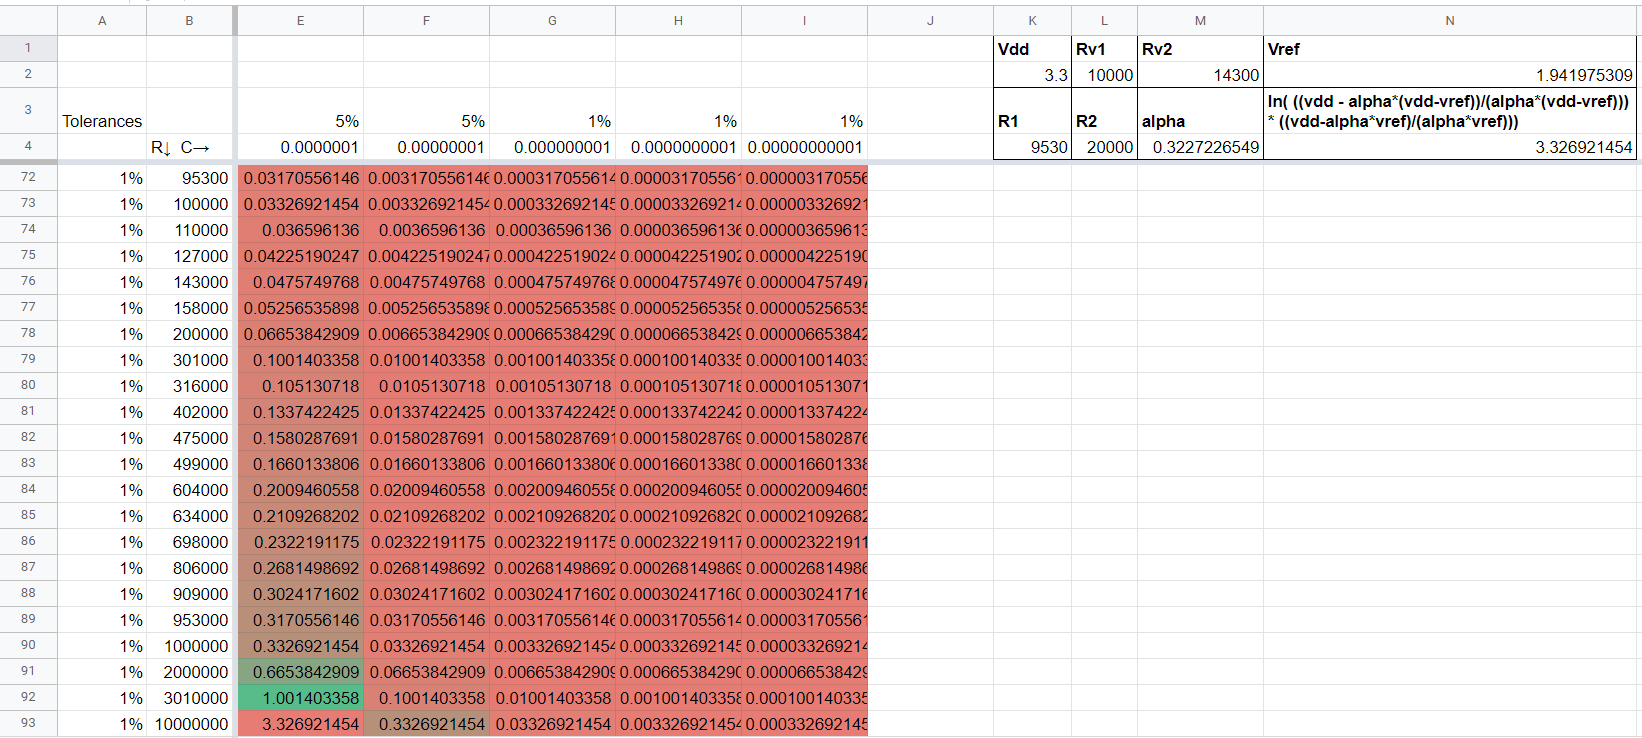
\includegraphics[width=.9\columnwidth]{images/spreadsheet.png}
    \caption{A screenshot of part of the spreadsheet used for calculating the period. The calculated period for the selected values is in cell E92.}
    \label{fig:spreadsheet}
\end{figure}

I avoided using the two largest capacitor values, since their high tolerance range of \(\pm10\%\) would leave me little room for other component variation. With that limitation, the closest period to 1 second was about 0.66 seconds using \(R_3=\qty{3.01}{\mega\ohm}\) and \(C_1=\qty{0.1}{\micro\farad}\). I then decreased alpha to around 0.32 by using \(R_4=\qty{9530}{\ohm}\) and \(R_5=\qty{20}{\kilo\ohm}\), which brought the period closer to \qty{1}{\second} (approx \qty{0.99}{\second}). I then increased \(V_{ref}\) to around \qty{1.94}{\volt} using \(R_1=\qty{10}{\kilo\ohm}\) and \(R_2=\qty{14.3}{\kilo\ohm}\), which brought the nominal period to \qty{1.00140}{\second}. I figured this would be close enough to try worst-case analysis.

\section{Worst-Case Tolerance Analysis in LTspice}

\begin{figure}[!ht]
    \centering
    \includesvg[width=.75\columnwidth]{images/spice_schem.svg}
    \caption{The schematic constructed in LTspice for simulation.}
    \label{fig:spice_schem}
\end{figure}

To determine whether the component values would satisfy the tolerance requirement, I simulated my circuit in LTspice (Figure~\ref{fig:spice_schem}) for every combination of the most extreme tolerance variations for each component. I did not include the voltage regulator in the simulation. I processed the resulting data in MATLAB to extract the longest and shortest period from the simulations. The code used can be found in Appendix~\ref{code}. The results showed the range of the periods to be \(\lbrack \qty{0.9309}{\second}, \qty{1.0733}{\second}\rbrack\), which is within \(\pm10\%\) of 1 second.

\appendix
\section{MATLAB Code}\label{code}
The following code extracts the longest and shortest oscillation periods from LTspice simulation output. Line 6 obtains a the highest value in the differential of the list of times where \(dV/dt>1000\) (all up-going transitions of the oscillation), which is the period.

\begin{minted}[linenos]{MATLAB}
loadspice('simulation.txt');
periods = zeros(1,length(time));
for i=1:length(time)
    t = time{1,i};
    v = vout{1,i};
    periods(i)=max(diff(t((diff(v)./diff(t))>1000)));
end
min(periods)
max(periods)
\end{minted}

\end{document}
